% !TeX encoding=utf8
% !TeX spellcheck = de_DE
% !TeX root = ../Diploma.tex

\chapter{Konzept des Servers}\label{sec:conceptServer}
Inhalt dieses Kapitels soll die Planung sein, welche für die Umsetzung des RESTful Schachservers benötigt wird. Dabei dient der erste Abschnitt für eine Erläuterung der Anforderungen, welche der Server mitbringen bzw. erfüllen soll. Enthalten ist dabei auch eine Erläuterung der benötigten Ressource. Im zweiten Abschnitt dieses Kapitels befasst sich anschließend damit, wie der Zugriff auf einzelne Ressourcen des REST-Server erfolgen soll. Dabei werden alle möglichen Request-Methoden für die jeweiligen Ressourcen näher beleuchtet.

\section{Anforderungen}\label{sec:anforderungen}
Die Grundanforderungen an den RESTful Schachserver sollen in erster Linie die Bereitstellung aller benötigten Ressourcen sein. Dabei sollen Elemente erstellt, ggf. bearbeitet und gelöscht werden können. Zusätzlich soll die Möglichkeit bestehen, einzelne oder alle gespeicherten Elemente einer Ressource abzufragen. Beim erstellen eines neuen Ressourcenelements soll dieses in einer SQLite Datenbank gespeichert und die ID automatisch durch SQLite generiert werden.\\
\\
Um ein Schachspiel abzubilden bedarf es dabei der Ressourcen Player (Spieler), Match (Partie) und Draw (Zug), welche in den nachfolgenden \hyperref[sec:resplayer, sec:resdraw]{Unterabschnitten~\ref{sec:resplayer} bis \ref{sec:resdraw}} näher betrachtet werden.\\
\\
Als abschließende Anforderung ist noch die Fehlerresistenz zu erwähnen. Denn die im Rahmen dieser Arbeit entstandene Praktikumsaufgabe \todo[inline]{Verweis auf Praktikumsaufgabe im Anhang} soll durch zukünftige Studenten absolviert werden, wobei der Server als Grundlage dienen soll.\\
\\
Zur Unterstützung der Erläuterungen in den \hyperref[sec:resplayer, sec:resdraw]{Kapiteln~\ref{sec:resplayer} bis \ref{sec:resdraw}} bietet die \hyperref[fig:classdiagram]{Abbildung~\ref{fig:classdiagram}}, in Form eines \gls{UML} Klassendiagramms, eine Veranschaulichung.
\begin{sidewaysfigure}
	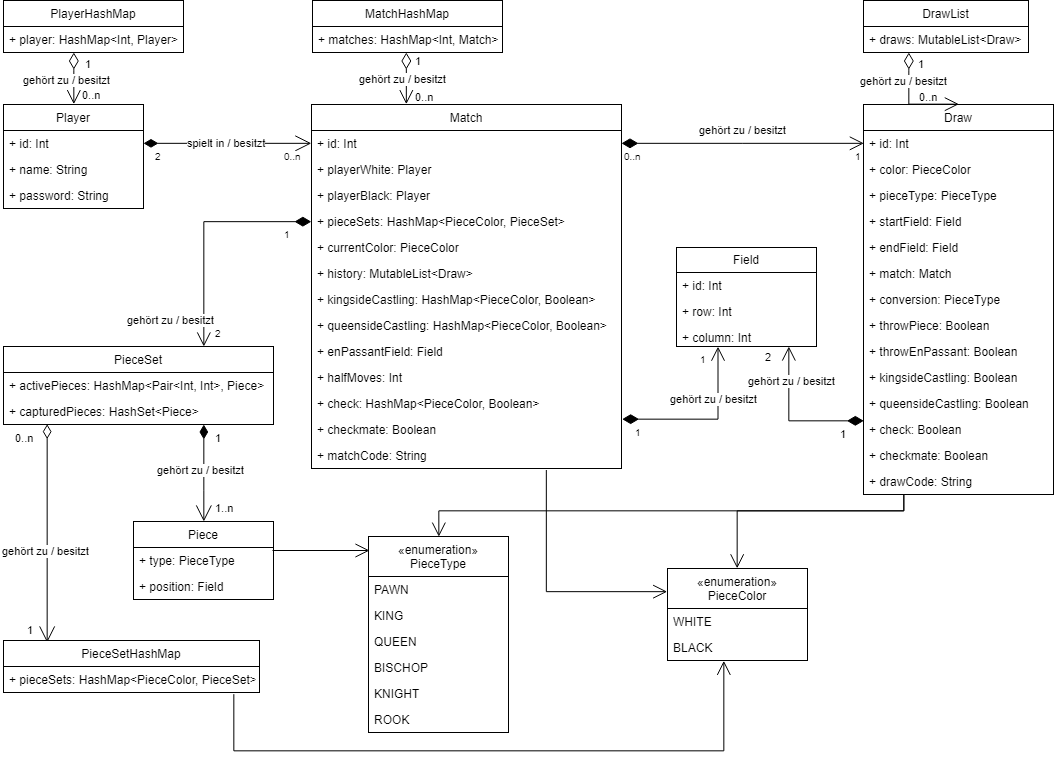
\includegraphics[width=0.9\textwidth]{images/classdiagram.png}
	\caption{Klassendiagramm: Modelle des Servers}
	\label{fig:classdiagram}
\end{sidewaysfigure}

\subsection{Ressource: Player (Spieler)}\label{sec:resplayer}
Neben der ID, welche schon im Abschnitt \ref{sec:anforderungen} erwähnt und durch die SQLite Datenbank generiert werden soll, besitzt der Player noch Informationen über seinen Name und sein Passwort.\\
\\
Nach dem anlegen eines neuen Players soll eine Änderung des Namens nicht gestattet sein, die des Passwortes hingegen schon.

\subsection{Ressource: Match (Partie)}\label{sec:resmatch}
Neben der ID besitzt ein Match Informationen über die beiden Spielteilnehmer und deren Figurenstellung auf dem Schachbrett. Zusätzlich wird registriert welcher der beiden Player als nächstes seinen nächsten Zug tätigen muss, welche Möglichkeiten zum rochieren bestehen, ob ein Schlag \enquote{en passant} möglich ist und wenn ja auf welches Feld gezogen werden muss und wie viele Halbzüge gespielt wurden. Der Wert der Halbzüge wird zurückgesetzt sobald eine Bauernfigur gezogen oder eine beliebige Figur geschmissen wurde. Zusätzlich kann über ein Match ermittelt werden ob ein Spieler im Schach steht oder ob das Spiel schon bis zum Schachmatt gespielt wurde. All diese Informationen werden zusätzlich noch als String in der \gls{FEN}\footnote{\label{foot:chapter}siehe \hyperref[sec:chessNotation]{Kapitel~\ref{sec:chessNotation}}} gespeichert.

\subsection{Ressource: Draw (Zug)}\label{sec:resdraw}
Die Ressource Draw speichert zusätzlich zur ID die Farbe des Spielers, die Art der Spielfigur, Start- und Endfeld des Zuges, ob eine Figur geschlagen wurde, wenn ja ob durch en passant und ob seitens der Dame oder des König rochiert wurde. Die Informationen werden ähnlich zum Match als String gespeichert, aber in diesem Fall in der \gls{SAN}\footref{foot:chapter}.

\section{Ressourcenzugriffe mithilfe von Controllern}
Die einzelnen Zugriffe auf die Ressourcen werden in den \hyperref[sec:playerController, sec:drawController]{Kapiteln~\ref{sec:playerController} bis \ref{sec:drawController}} nach ihrer Art bzw. deren Aufgaben in einzelne Controller unterteilt, um eine gute Übersicht zu wahren. Für alle Einstiegspunkte der \gls{REST}-\gls{API} soll die Request-Methode \enquote{OPTIONS} bereitstehen, über welchen ermittelt werden kann welche Methoden für den jeweiligen Einstiegspunkt zur Verfügung stehen.\\
\\
Etwaige Requestparameter sollen in dem Format \gls{JSON} oder x-www-form-urlencode mitgeschickt werden können. Die gesendeten Anfragen sollen ihr Feedback je nach Wunsch, via Content Negotiation, entweder in \gls{JSON} oder in \gls{XML} zurücksenden. Dabei sollen drei Strategien bereitgestellt werden, entweder mittels Suffix, einem URL-Parameter oder dem \gls{HTTP} Accept-Header. 

\subsection{Player Controller}\label{sec:playerController}
Der Player Controller soll zwei Einstiegspunkt an den \glspl{URI} \code{/player/} und \code{/player/\{id\}} zur Verfügung stellen. Der Parameter \code{\{id\}} dient dabei als Platzhalter für die ID eines Players, welche wiederum als Zahl dargestellt wird.\\
\\
Am ersten Einstiegspunkt soll eine Liste aller Spieler über einen GET-Request bereitgestellt werden können. Des weiteren soll an diesem die Möglichkeit bestehen einen neuen Player mithilfe eines POST-Requests zu erzeugen. Dabei muss als Parameter der Name und das Passwort des Players mitgegeben werden. Die SQLite-Datenbank soll die ID dabei automatisch mittels Autoincrement erzeugen. Bei erfolgreicher Erstellung des Players soll dieser zurückgegeben werden, ansonsten \code{NULL}.\\
\\
Am zweiten Einstiegspunkt soll ein einzelner existierender Player über einen GET-Request bereitgestellt, über einen DELETE-Request gelöscht und über einen PATCH-Request aktualisiert werden können. Nur das Passwort darf dabei laut Anforderungen\footnote{siehe \hyperref[sec:anforderungen]{Kapitel~\ref{sec:anforderungen}}} aktualisiert werden, wobei dieses zusätzlich als Parameter an den Request mit angehangen werden muss.\\
\\
Für ein besseres Verständnis bietet die \hyperref[fig:playerController]{Abbildung~\ref{fig:playerController}} eine visuelle Verdeutlichung der Einstiegspunkte des Player Controllers.
\begin{figure}[htb]
	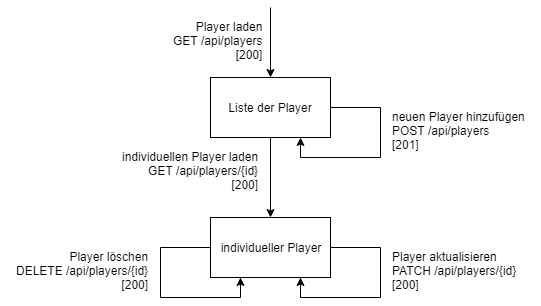
\includegraphics[width=0.7\textwidth]{images/player-controller.png}
	\caption{Player Controller - Übersicht der Einstiegspunkte}
	\label{fig:playerController}
\end{figure}

\subsection{Match Controller}\label{sec:matchController}
Die \glspl{URI} \code{/match/}, \code{/match/\{id\}}, \code{/match/{id}/draws} und \code{/match/{id}/pieceSets} sollen durch den Match Controller bereitgestellt werden.\\
\\
Dabei soll die erste \gls{URI} ebenso wie beim \enquote{Player Controller} Zurverfügungstellung einer Liste aller registrierten Matches und dem anlegen neuer dienen. Das Bereitstellen der Liste soll mittels GET- und das anlegen mittels POST-Request erfolgen. Der GET-Request soll zwei optionale boolesche Parameter bereitstellen, womit das Senden der Historie von Draws bzw. der Figurenstellung bestimmt werden soll. Standardmäßig sollen dabei die Parameter \code{TRUE} sein. Weiter unten in diesem Kapitel wird beschrieben wie diese Informationen separat geholt werden können. Um ein neues Match zu registrieren, müssen dabei die ID's der beiden Spielteilnehmer mitgeschickt werden. Anhand des Parameternamens soll festgelegt werden welcher Spieler Weiß und welcher Schwarz spielen soll.\\
\\
Der zweite Einstiegspunkt soll in diesem Controller ausschließlich dazu verwendet werden, um einzelne Matches mithilfe eines GET-Request anzufordern oder mithilfe eines DELETE-Request zu löschen. Für das anfordern eines einzelnen Matches stehen ebenso zwei boolesche, wie beim Anfordern einer Liste, bereit. Wenn ein Nutzer ein Match löscht, sollen ebenfalls alle zugehörigen Draws gelöscht werden. Um eine unrechtmäßige Manipulation der Match-Daten durch einen Nutzer zu verhindern, soll keine Möglichkeit bereitstehen ein Match zu aktualisieren. Die Aktualisierung eines Matches soll ausschließlich durch das hinzufügen von Draws erfolgen.\footnote{siehe \hyperref[sec:drawController]{Kapitel~\ref{sec:drawController}}}\\
\\
Die letzten beiden Einstiegspunkte sollen dazu dienen große Match bezogene Daten separat zu ermitteln. Dabei soll mittels GET-Request an der \gls{URI} \code{/match/{id}/draw} eine Liste aller Draws und über die \gls{URI} \code{/match/{id}/pieceSets} eine Map mit allen Figuren der beiden Spielteilnehmer bereitgestellt werden. Neben den aktuell auf dem Spielfeld stehenden Figuren sollen dabei auch die geschmissen mitgeschickt werden.\\
\\
Die \hyperref[fig:matchController]{Abbildung~\ref{fig:matchController}} bietet für die zuvor definierten Einstiegspunkte eine grafische Veranschaulichung.
\begin{figure}[htb]
	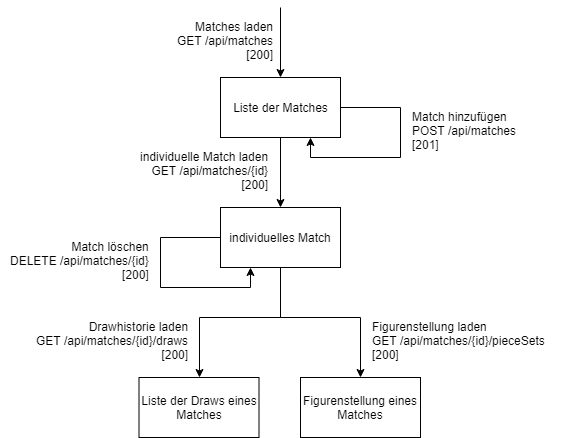
\includegraphics[width=0.7\textwidth]{images/match-controller.png}
	\caption{Match Controller - Übersicht der Einstiegspunkte}
	\label{fig:matchController}
\end{figure}

\subsection{Draw Controller}\label{sec:drawController}
Auch der Draw Controller stellt wieder zwei Einstiegspunkte an den \glspl{URI} \code{/draw/} und \code{/draw/\{id\}} bereit. \\
\\
Am ersten Einstiegspunkt soll wieder das bereitstellen einer Liste mittels GET- und das hinzufügen mittels POST-Request von Draws zur Verfügung gestellt werden. Für das hinzufügen eines neuen Draws ist die ID des Matches und der Draw-Code in der \gls{SAN} als Parameter von nöten. Zusätzlich soll die Möglichkeit bestehen die Zeilen- und die Spaltennummer der Startposition mitzugeben. Wenn diese Informationen nicht mitgegeben werden, so soll der Controller die Startposition kalkulieren. Spalten sollen dabei als Nummern und nicht als Buchstaben mitgegeben werden\footnote{A $\rightarrow$ 8; ...; H $\rightarrow$ 8}. Nach erfolgreicher Validierung des Draw-Codes soll der Draw dem zugehörigen Match hinzugefügt und die Match-Daten aktualisiert werden.\\
\\
Über den zweiten Einstiegspunkt soll wieder die Abfrage nach einem einzelnen Draw möglich sein. Eine Möglichkeit zum Löschen oder Aktualisieren des Draws soll nicht bestehen, da sonst der Nutzer wieder eine Möglichkeit hätte das Match zu manipulieren. Das Löschen von Draws soll über die Löschung des dazugehörigen Matches erfolgen\footnote{siehe \hyperref[sec:matchController]{Kapitel~\ref{sec:matchController}}}.\\
\\
Wie in den vorherigen Kapiteln bietet die \hyperref[fig:drawController]{Abbildung~\ref{fig:drawController}} ein Veranschaulichung.
\begin{figure}[htb]
	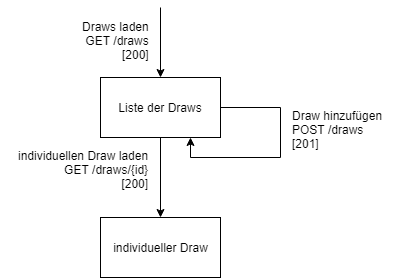
\includegraphics[width=0.54\textwidth]{images/draw-controller.png}
	\caption{Draw Controller - Übersicht der Einstiegspunkte}
	\label{fig:drawController}
\end{figure}